\documentclass[]{book}
\usepackage{lmodern}
\usepackage{amssymb,amsmath}
\usepackage{ifxetex,ifluatex}
\usepackage{fixltx2e} % provides \textsubscript
\ifnum 0\ifxetex 1\fi\ifluatex 1\fi=0 % if pdftex
  \usepackage[T1]{fontenc}
  \usepackage[utf8]{inputenc}
\else % if luatex or xelatex
  \ifxetex
    \usepackage{mathspec}
  \else
    \usepackage{fontspec}
  \fi
  \defaultfontfeatures{Ligatures=TeX,Scale=MatchLowercase}
\fi
% use upquote if available, for straight quotes in verbatim environments
\IfFileExists{upquote.sty}{\usepackage{upquote}}{}
% use microtype if available
\IfFileExists{microtype.sty}{%
\usepackage{microtype}
\UseMicrotypeSet[protrusion]{basicmath} % disable protrusion for tt fonts
}{}
\usepackage[margin=1in]{geometry}
\usepackage{hyperref}
\hypersetup{unicode=true,
            pdftitle={R you ready?},
            pdfauthor={Reto Wyss, Greg Martin},
            pdfborder={0 0 0},
            breaklinks=true}
\urlstyle{same}  % don't use monospace font for urls
\usepackage{natbib}
\bibliographystyle{apalike}
\usepackage{color}
\usepackage{fancyvrb}
\newcommand{\VerbBar}{|}
\newcommand{\VERB}{\Verb[commandchars=\\\{\}]}
\DefineVerbatimEnvironment{Highlighting}{Verbatim}{commandchars=\\\{\}}
% Add ',fontsize=\small' for more characters per line
\usepackage{framed}
\definecolor{shadecolor}{RGB}{248,248,248}
\newenvironment{Shaded}{\begin{snugshade}}{\end{snugshade}}
\newcommand{\KeywordTok}[1]{\textcolor[rgb]{0.13,0.29,0.53}{\textbf{#1}}}
\newcommand{\DataTypeTok}[1]{\textcolor[rgb]{0.13,0.29,0.53}{#1}}
\newcommand{\DecValTok}[1]{\textcolor[rgb]{0.00,0.00,0.81}{#1}}
\newcommand{\BaseNTok}[1]{\textcolor[rgb]{0.00,0.00,0.81}{#1}}
\newcommand{\FloatTok}[1]{\textcolor[rgb]{0.00,0.00,0.81}{#1}}
\newcommand{\ConstantTok}[1]{\textcolor[rgb]{0.00,0.00,0.00}{#1}}
\newcommand{\CharTok}[1]{\textcolor[rgb]{0.31,0.60,0.02}{#1}}
\newcommand{\SpecialCharTok}[1]{\textcolor[rgb]{0.00,0.00,0.00}{#1}}
\newcommand{\StringTok}[1]{\textcolor[rgb]{0.31,0.60,0.02}{#1}}
\newcommand{\VerbatimStringTok}[1]{\textcolor[rgb]{0.31,0.60,0.02}{#1}}
\newcommand{\SpecialStringTok}[1]{\textcolor[rgb]{0.31,0.60,0.02}{#1}}
\newcommand{\ImportTok}[1]{#1}
\newcommand{\CommentTok}[1]{\textcolor[rgb]{0.56,0.35,0.01}{\textit{#1}}}
\newcommand{\DocumentationTok}[1]{\textcolor[rgb]{0.56,0.35,0.01}{\textbf{\textit{#1}}}}
\newcommand{\AnnotationTok}[1]{\textcolor[rgb]{0.56,0.35,0.01}{\textbf{\textit{#1}}}}
\newcommand{\CommentVarTok}[1]{\textcolor[rgb]{0.56,0.35,0.01}{\textbf{\textit{#1}}}}
\newcommand{\OtherTok}[1]{\textcolor[rgb]{0.56,0.35,0.01}{#1}}
\newcommand{\FunctionTok}[1]{\textcolor[rgb]{0.00,0.00,0.00}{#1}}
\newcommand{\VariableTok}[1]{\textcolor[rgb]{0.00,0.00,0.00}{#1}}
\newcommand{\ControlFlowTok}[1]{\textcolor[rgb]{0.13,0.29,0.53}{\textbf{#1}}}
\newcommand{\OperatorTok}[1]{\textcolor[rgb]{0.81,0.36,0.00}{\textbf{#1}}}
\newcommand{\BuiltInTok}[1]{#1}
\newcommand{\ExtensionTok}[1]{#1}
\newcommand{\PreprocessorTok}[1]{\textcolor[rgb]{0.56,0.35,0.01}{\textit{#1}}}
\newcommand{\AttributeTok}[1]{\textcolor[rgb]{0.77,0.63,0.00}{#1}}
\newcommand{\RegionMarkerTok}[1]{#1}
\newcommand{\InformationTok}[1]{\textcolor[rgb]{0.56,0.35,0.01}{\textbf{\textit{#1}}}}
\newcommand{\WarningTok}[1]{\textcolor[rgb]{0.56,0.35,0.01}{\textbf{\textit{#1}}}}
\newcommand{\AlertTok}[1]{\textcolor[rgb]{0.94,0.16,0.16}{#1}}
\newcommand{\ErrorTok}[1]{\textcolor[rgb]{0.64,0.00,0.00}{\textbf{#1}}}
\newcommand{\NormalTok}[1]{#1}
\usepackage{longtable,booktabs}
\usepackage{graphicx,grffile}
\makeatletter
\def\maxwidth{\ifdim\Gin@nat@width>\linewidth\linewidth\else\Gin@nat@width\fi}
\def\maxheight{\ifdim\Gin@nat@height>\textheight\textheight\else\Gin@nat@height\fi}
\makeatother
% Scale images if necessary, so that they will not overflow the page
% margins by default, and it is still possible to overwrite the defaults
% using explicit options in \includegraphics[width, height, ...]{}
\setkeys{Gin}{width=\maxwidth,height=\maxheight,keepaspectratio}
\IfFileExists{parskip.sty}{%
\usepackage{parskip}
}{% else
\setlength{\parindent}{0pt}
\setlength{\parskip}{6pt plus 2pt minus 1pt}
}
\setlength{\emergencystretch}{3em}  % prevent overfull lines
\providecommand{\tightlist}{%
  \setlength{\itemsep}{0pt}\setlength{\parskip}{0pt}}
\setcounter{secnumdepth}{5}
% Redefines (sub)paragraphs to behave more like sections
\ifx\paragraph\undefined\else
\let\oldparagraph\paragraph
\renewcommand{\paragraph}[1]{\oldparagraph{#1}\mbox{}}
\fi
\ifx\subparagraph\undefined\else
\let\oldsubparagraph\subparagraph
\renewcommand{\subparagraph}[1]{\oldsubparagraph{#1}\mbox{}}
\fi

%%% Use protect on footnotes to avoid problems with footnotes in titles
\let\rmarkdownfootnote\footnote%
\def\footnote{\protect\rmarkdownfootnote}

%%% Change title format to be more compact
\usepackage{titling}

% Create subtitle command for use in maketitle
\newcommand{\subtitle}[1]{
  \posttitle{
    \begin{center}\large#1\end{center}
    }
}

\setlength{\droptitle}{-2em}

  \title{R you ready?}
    \pretitle{\vspace{\droptitle}\centering\huge}
  \posttitle{\par}
    \author{Reto Wyss, Greg Martin}
    \preauthor{\centering\large\emph}
  \postauthor{\par}
      \predate{\centering\large\emph}
  \postdate{\par}
    \date{2018-10-31}

\usepackage{booktabs}

\usepackage{amsthm}
\newtheorem{theorem}{Theorem}[chapter]
\newtheorem{lemma}{Lemma}[chapter]
\theoremstyle{definition}
\newtheorem{definition}{Definition}[chapter]
\newtheorem{corollary}{Corollary}[chapter]
\newtheorem{proposition}{Proposition}[chapter]
\theoremstyle{definition}
\newtheorem{example}{Example}[chapter]
\theoremstyle{definition}
\newtheorem{exercise}{Exercise}[chapter]
\theoremstyle{remark}
\newtheorem*{remark}{Remark}
\newtheorem*{solution}{Solution}
\let\BeginKnitrBlock\begin \let\EndKnitrBlock\end
\begin{document}
\maketitle

{
\setcounter{tocdepth}{1}
\tableofcontents
}
\chapter*{Preface}\label{preface}
\addcontentsline{toc}{chapter}{Preface}

\begin{figure}
\includegraphics[width=1\linewidth]{static/images/test-cover} \caption{RStudio (This is the caption)}\label{fig:asd-view}
\end{figure}

\[
a = \sum
\]

In this book \citet{R-base} and \citet{R-tidyverse}

\BeginKnitrBlock{definition}
\protect\hypertarget{def:unnamed-chunk-3}{}{\label{def:unnamed-chunk-3}
}Here is my theorem.
\EndKnitrBlock{definition}

\BeginKnitrBlock{example}
\protect\hypertarget{exm:My-Example}{}{\label{exm:My-Example} }This is my
example
\EndKnitrBlock{example}

\begin{foo}
This is a custom block. We can style it however we want.
\end{foo}

\chapter{Setup}\label{setup}

In this chapter bla bla (promise)

(preview)

\section{Installing R and RStudio}\label{installing-r-and-rstudio}

\begin{itemize}
\tightlist
\item
  R \url{https://cran.r-project.org/mirrors.html}
\item
  RStudio \url{https://www.rstudio.com/products/rstudio/download/}
\end{itemize}

\chapter{Working with R in RStudio}\label{working-with-r-in-rstudio}

In this chapter bla bla (promise)

(preview)

Explain Quadrants

\begin{quote}
I think we could create a section for each of the important
windows/tabs. Also we should make every step as actionable as possible.
\end{quote}

Testing image

\begin{figure}
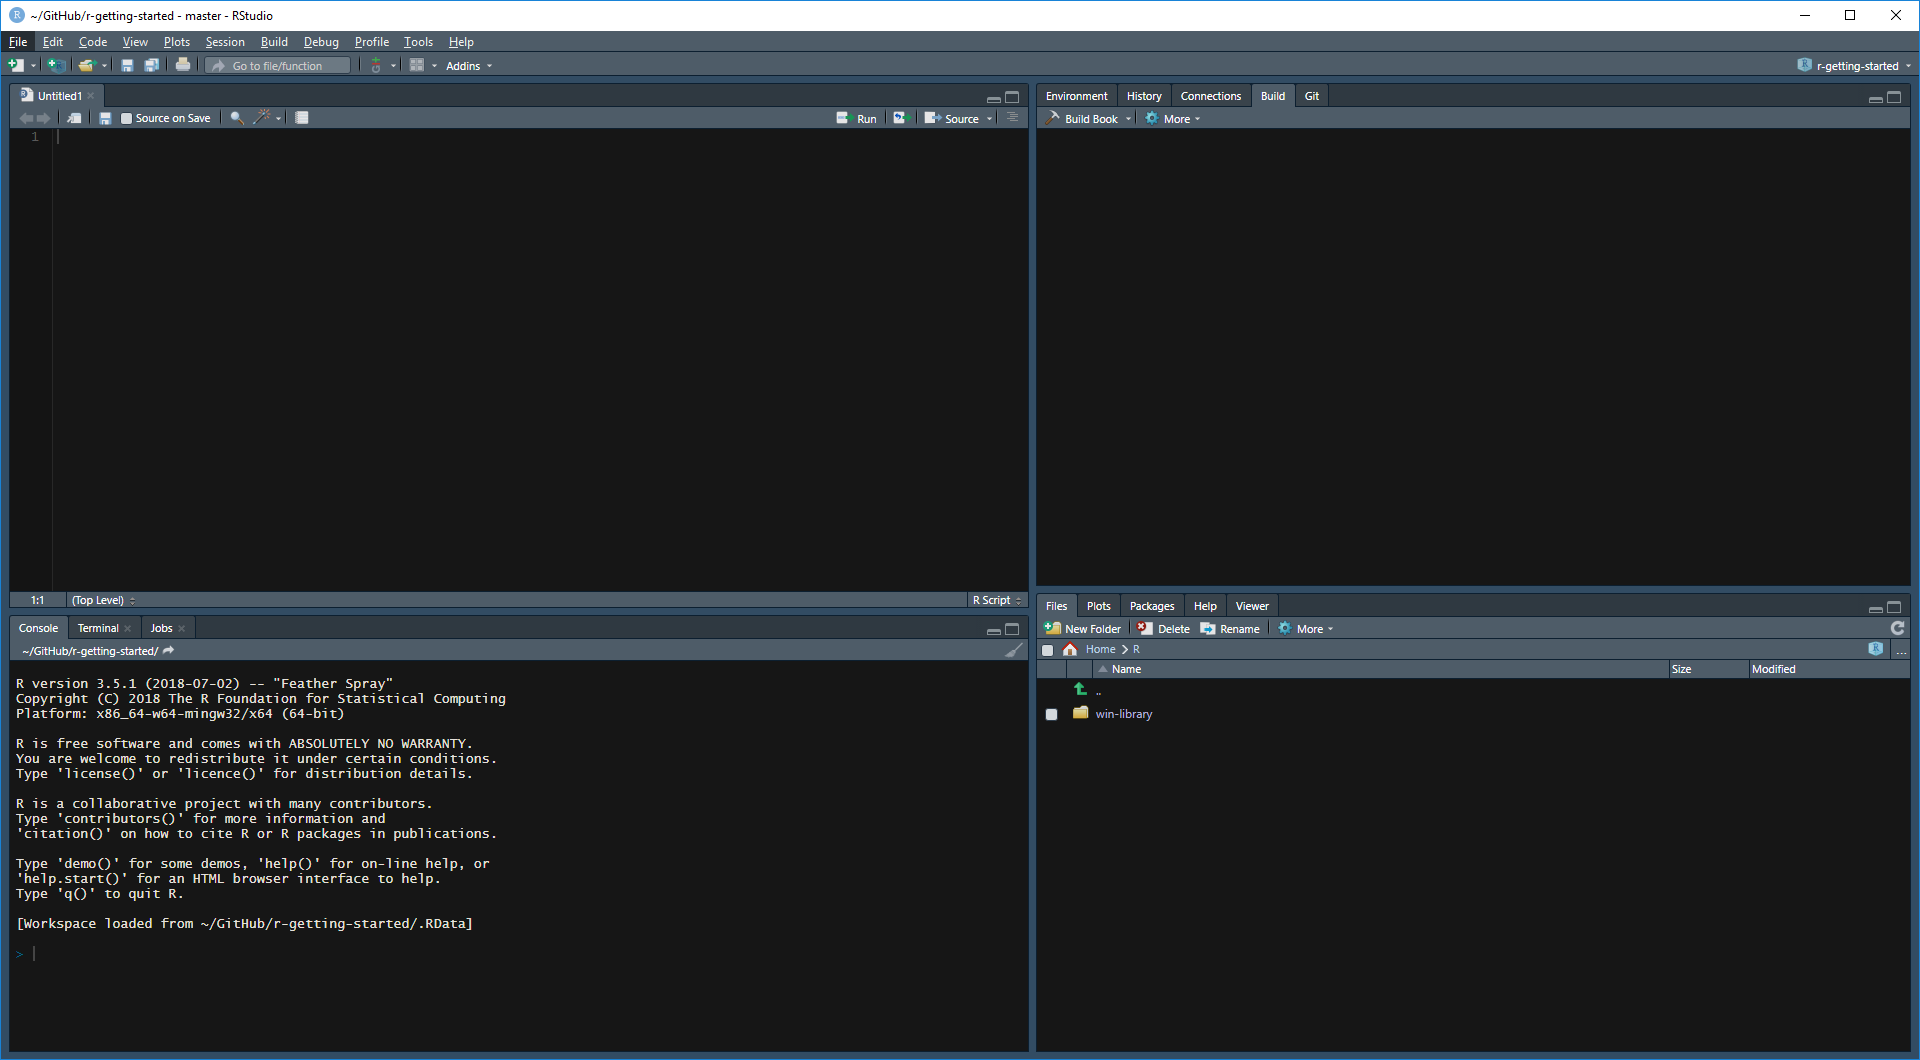
\includegraphics[width=1\linewidth]{static/images/RStudio} \caption{RStudio (This is the caption)}\label{fig:rstudio-view}
\end{figure}

\section{Files, Viewer, Help (br)}\label{files-viewer-help-br}

\section{The Console (bl)}\label{the-console-bl}

\begin{quote}
{[}Action{]} Show arthimetic ops here
\end{quote}

Now that you are all set up we want to dive straight into using R. To
get the most out of this tutorial you should try to run the code
yourself on the console in RStudio. You can think of R as a calculator -
a very powerful calculator. R supports the five basic arithmetic
operations you are familiar with and three more you might not yet have
seen. The operators for addition, subtraction and multiplication are
self explanatory.

\begin{Shaded}
\begin{Highlighting}[]
\DecValTok{4} \OperatorTok{+}\StringTok{ }\DecValTok{5}    \CommentTok{# Addition}
\DecValTok{10} \OperatorTok{-}\StringTok{ }\DecValTok{1}   \CommentTok{# Subtraction}
\DecValTok{3} \OperatorTok{*}\StringTok{ }\DecValTok{3}    \CommentTok{# Multiplication}
\DecValTok{27} \OperatorTok{/}\StringTok{ }\DecValTok{3}   \CommentTok{# Division}
\DecValTok{3} \OperatorTok{**}\StringTok{ }\DecValTok{2}   \CommentTok{# Power}

\CommentTok{# Standard operator presedence and parentheses rules apply}
\NormalTok{(}\DecValTok{35} \OperatorTok{+}\StringTok{ }\DecValTok{8}\NormalTok{) }\OperatorTok{*}\StringTok{ }\DecValTok{2} \OperatorTok{**}\StringTok{ }\NormalTok{(}\DecValTok{10} \OperatorTok{/}\StringTok{ }\DecValTok{2}\NormalTok{) }\OperatorTok{-}\StringTok{ }\DecValTok{39}
\end{Highlighting}
\end{Shaded}

\begin{verbatim}
## [1] 9
## [1] 9
## [1] 9
## [1] 9
## [1] 9
## [1] 1337
\end{verbatim}

There are two ways of writing the power operator \texttt{**} and
\texttt{\^{}}. Personally, I prefer the first way.

\begin{quote}
Maybe cut this part
\end{quote}

Now, let's have a look at the three less common operator. They are
modulo, whole number division and matrix-multiplication. test change

\begin{Shaded}
\begin{Highlighting}[]
\DecValTok{43} \OperatorTok\StringTok{ }\DecValTok{7}               \CommentTok{# Modulo}
\DecValTok{43} \OperatorTok\StringTok{ }\DecValTok{7}              \CommentTok{# Whole number division}
\KeywordTok{c}\NormalTok{(}\DecValTok{4}\NormalTok{, }\DecValTok{2}\NormalTok{) }\OperatorTok\StringTok{ }\KeywordTok{c}\NormalTok{(}\DecValTok{2}\NormalTok{, }\DecValTok{4}\NormalTok{)   }\CommentTok{# Matrix-multiplication}
\end{Highlighting}
\end{Shaded}

\begin{verbatim}
## [1] 1
## [1] 6
##      [,1]
## [1,]   16
\end{verbatim}

\section{Script (tl)}\label{script-tl}

\begin{quote}
{[}Action{]} Show how code (arithmetic can be written in a script file
and then be executed on the console)
\end{quote}

Top left is the script window

\section{History and Environment (tr)}\label{history-and-environment-tr}

\begin{quote}
{[}Action{]} Show how to assign variables
\end{quote}

ow, let's define our first variable. We will call it
\texttt{my\_first\_variable}.

\subsection{Creating variables}\label{creating-variables}

\begin{Shaded}
\begin{Highlighting}[]
\NormalTok{my_first_variable <-}\StringTok{ }\DecValTok{42}
\end{Highlighting}
\end{Shaded}

When you enter this on your R console in RStudio nothing will happen. We
have told R to store the number 42 in a variable and we call this
specific variable \texttt{my\_first\_variable}. To retrieve the value of
our variable we just type the variable name and hit enter.

\begin{Shaded}
\begin{Highlighting}[]
\NormalTok{my_first_variable}
\end{Highlighting}
\end{Shaded}

\begin{verbatim}
## [1] 42
\end{verbatim}

Arithmetic operations work on variables just like they do on literal
numbers.

\begin{Shaded}
\begin{Highlighting}[]
\NormalTok{a <-}\StringTok{ }\DecValTok{5}
\NormalTok{b <-}\StringTok{ }\DecValTok{10}
\NormalTok{a }\OperatorTok{*}\StringTok{ }\NormalTok{b}
\end{Highlighting}
\end{Shaded}

\begin{verbatim}
## [1] 50
\end{verbatim}

\subsection{Vectors}\label{vectors}

Vectors are a data-structure. They can hold multiple values at once and
they can be referenced by a single variable. To create a vector you will
use \texttt{c()}.

\begin{Shaded}
\begin{Highlighting}[]
\NormalTok{my_first_vector <-}\StringTok{ }\KeywordTok{c}\NormalTok{(}\DecValTok{42}\NormalTok{, }\DecValTok{5}\NormalTok{, }\DecValTok{10}\NormalTok{)}
\end{Highlighting}
\end{Shaded}

You can have a glimpse at the values in your vector by typing its name.

\begin{Shaded}
\begin{Highlighting}[]
\NormalTok{my_first_vector}
\end{Highlighting}
\end{Shaded}

\begin{verbatim}
## [1] 42  5 10
\end{verbatim}

Performing arithmetics on vector is analogous to atomic values.

\begin{Shaded}
\begin{Highlighting}[]
\NormalTok{my_first_vector }\OperatorTok{*}\StringTok{ }\DecValTok{10}
\end{Highlighting}
\end{Shaded}

\begin{verbatim}
## [1] 420  50 100
\end{verbatim}

\chapter{Starting Data Analysis}\label{starting-data-analysis}

\section{Creating A Project}\label{creating-a-project}

You should always use the project functonality when you work with R and
RStudio.

This also sets the working-directory.

\begin{Shaded}
\begin{Highlighting}[]
\KeywordTok{getwd}\NormalTok{()}
\end{Highlighting}
\end{Shaded}

\begin{verbatim}
## [1] "/Users/GregMartin/Dropbox/R/Books/R-Getting-Started/r-getting-started"
\end{verbatim}

\section{Folder Structure}\label{folder-structure}

\begin{quote}
Show new and existing directory options. Some people may already have
collected data.
\end{quote}

\begin{verbatim}
+---Data
|
+---Output
\end{verbatim}

\section{Packages}\label{packages}

\begin{quote}
We can prime this by telling people about the R community in the
introduction
\end{quote}

installing and loading (maybe show updating in RStudio)

\section{Importing Data}\label{importing-data}

\begin{quote}
This is rather short and not worth a chapter on it's own.
\end{quote}

Filetypes:

\begin{itemize}
\tightlist
\item
  csv
\item
  xlsx
\end{itemize}

\begin{Shaded}
\begin{Highlighting}[]
\KeywordTok{library}\NormalTok{(readr)}
\end{Highlighting}
\end{Shaded}

Here we introduce the \texttt{readr} and \texttt{readxl} packagtes.

\begin{Shaded}
\begin{Highlighting}[]
\NormalTok{my_iris <-}\StringTok{ }\KeywordTok{read_csv}\NormalTok{(}\StringTok{"iris.csv"}\NormalTok{)}
\end{Highlighting}
\end{Shaded}

\begin{verbatim}
## Parsed with column specification:
## cols(
##   Sepal.Length = col_double(),
##   Sepal.Width = col_double(),
##   Petal.Length = col_double(),
##   Petal.Width = col_double(),
##   Species = col_character()
## )
\end{verbatim}

\begin{Shaded}
\begin{Highlighting}[]
\KeywordTok{head}\NormalTok{(my_iris, }\DataTypeTok{n =} \DecValTok{5}\NormalTok{)}
\end{Highlighting}
\end{Shaded}

\begin{verbatim}
## # A tibble: 5 x 5
##   Sepal.Length Sepal.Width Petal.Length Petal.Width Species
##          <dbl>       <dbl>        <dbl>       <dbl>   <chr>
## 1          5.1         3.5          1.4         0.2  setosa
## 2          4.9         3.0          1.4         0.2  setosa
## 3          4.7         3.2          1.3         0.2  setosa
## 4          4.6         3.1          1.5         0.2  setosa
## 5          5.0         3.6          1.4         0.2  setosa
\end{verbatim}

this is useful because we can fix the column types like this.

\begin{Shaded}
\begin{Highlighting}[]
\NormalTok{my_iris <-}\StringTok{ }\KeywordTok{read_csv}\NormalTok{(}
    \DataTypeTok{file =} \StringTok{"iris.csv"}\NormalTok{,}
    \DataTypeTok{col_types =} \KeywordTok{cols}\NormalTok{(}
      \DataTypeTok{Sepal.Length =} \KeywordTok{col_double}\NormalTok{(),}
      \DataTypeTok{Sepal.Width =} \KeywordTok{col_double}\NormalTok{(),}
      \DataTypeTok{Petal.Length =} \KeywordTok{col_double}\NormalTok{(),}
      \DataTypeTok{Petal.Width =} \KeywordTok{col_double}\NormalTok{(),}
      \DataTypeTok{Species =} \KeywordTok{col_character}\NormalTok{()}
\NormalTok{    )}
\NormalTok{)}
\end{Highlighting}
\end{Shaded}

\chapter{Manipulating Data}\label{manipulating-data}

Here we introduce the \texttt{tidyr}, \texttt{dplyr}, \texttt{stringr}
and \texttt{forcats} packages.

Important functions:

\begin{itemize}
\tightlist
\item
  dplyr::rename
\item
  dplyr::mutate
\item
  tidyr::separate
\item
  stringr::str\_extract
\item
  stringr::str\_replace
\end{itemize}

\begin{Shaded}
\begin{Highlighting}[]
\KeywordTok{library}\NormalTok{(tidyr)}


\NormalTok{iris }\OperatorTok\StringTok{ }
\StringTok{  }\KeywordTok{separate}\NormalTok{(Sepal.Length, }\DataTypeTok{into =} \KeywordTok{c}\NormalTok{(}\StringTok{"first"}\NormalTok{, }\StringTok{"second"}\NormalTok{), }\DataTypeTok{sep =} \StringTok{"}\CharTok{\textbackslash{}\textbackslash{}}\StringTok{."}\NormalTok{)}
\end{Highlighting}
\end{Shaded}

\begin{verbatim}
## Warning: Too few values at 17 locations: 5, 8, 26, 27, 36, 41, 44, 50, 51,
## 61, 63, 79, 84, 86, 94, 120, 139
\end{verbatim}

\begin{verbatim}
##     first second Sepal.Width Petal.Length Petal.Width    Species
## 1       5      1         3.5          1.4         0.2     setosa
## 2       4      9         3.0          1.4         0.2     setosa
## 3       4      7         3.2          1.3         0.2     setosa
## 4       4      6         3.1          1.5         0.2     setosa
## 5       5   <NA>         3.6          1.4         0.2     setosa
## 6       5      4         3.9          1.7         0.4     setosa
## 7       4      6         3.4          1.4         0.3     setosa
## 8       5   <NA>         3.4          1.5         0.2     setosa
## 9       4      4         2.9          1.4         0.2     setosa
## 10      4      9         3.1          1.5         0.1     setosa
## 11      5      4         3.7          1.5         0.2     setosa
## 12      4      8         3.4          1.6         0.2     setosa
## 13      4      8         3.0          1.4         0.1     setosa
## 14      4      3         3.0          1.1         0.1     setosa
## 15      5      8         4.0          1.2         0.2     setosa
## 16      5      7         4.4          1.5         0.4     setosa
## 17      5      4         3.9          1.3         0.4     setosa
## 18      5      1         3.5          1.4         0.3     setosa
## 19      5      7         3.8          1.7         0.3     setosa
## 20      5      1         3.8          1.5         0.3     setosa
## 21      5      4         3.4          1.7         0.2     setosa
## 22      5      1         3.7          1.5         0.4     setosa
## 23      4      6         3.6          1.0         0.2     setosa
## 24      5      1         3.3          1.7         0.5     setosa
## 25      4      8         3.4          1.9         0.2     setosa
## 26      5   <NA>         3.0          1.6         0.2     setosa
## 27      5   <NA>         3.4          1.6         0.4     setosa
## 28      5      2         3.5          1.5         0.2     setosa
## 29      5      2         3.4          1.4         0.2     setosa
## 30      4      7         3.2          1.6         0.2     setosa
## 31      4      8         3.1          1.6         0.2     setosa
## 32      5      4         3.4          1.5         0.4     setosa
## 33      5      2         4.1          1.5         0.1     setosa
## 34      5      5         4.2          1.4         0.2     setosa
## 35      4      9         3.1          1.5         0.2     setosa
## 36      5   <NA>         3.2          1.2         0.2     setosa
## 37      5      5         3.5          1.3         0.2     setosa
## 38      4      9         3.6          1.4         0.1     setosa
## 39      4      4         3.0          1.3         0.2     setosa
## 40      5      1         3.4          1.5         0.2     setosa
## 41      5   <NA>         3.5          1.3         0.3     setosa
## 42      4      5         2.3          1.3         0.3     setosa
## 43      4      4         3.2          1.3         0.2     setosa
## 44      5   <NA>         3.5          1.6         0.6     setosa
## 45      5      1         3.8          1.9         0.4     setosa
## 46      4      8         3.0          1.4         0.3     setosa
## 47      5      1         3.8          1.6         0.2     setosa
## 48      4      6         3.2          1.4         0.2     setosa
## 49      5      3         3.7          1.5         0.2     setosa
## 50      5   <NA>         3.3          1.4         0.2     setosa
## 51      7   <NA>         3.2          4.7         1.4 versicolor
## 52      6      4         3.2          4.5         1.5 versicolor
## 53      6      9         3.1          4.9         1.5 versicolor
## 54      5      5         2.3          4.0         1.3 versicolor
## 55      6      5         2.8          4.6         1.5 versicolor
## 56      5      7         2.8          4.5         1.3 versicolor
## 57      6      3         3.3          4.7         1.6 versicolor
## 58      4      9         2.4          3.3         1.0 versicolor
## 59      6      6         2.9          4.6         1.3 versicolor
## 60      5      2         2.7          3.9         1.4 versicolor
## 61      5   <NA>         2.0          3.5         1.0 versicolor
## 62      5      9         3.0          4.2         1.5 versicolor
## 63      6   <NA>         2.2          4.0         1.0 versicolor
## 64      6      1         2.9          4.7         1.4 versicolor
## 65      5      6         2.9          3.6         1.3 versicolor
## 66      6      7         3.1          4.4         1.4 versicolor
## 67      5      6         3.0          4.5         1.5 versicolor
## 68      5      8         2.7          4.1         1.0 versicolor
## 69      6      2         2.2          4.5         1.5 versicolor
## 70      5      6         2.5          3.9         1.1 versicolor
## 71      5      9         3.2          4.8         1.8 versicolor
## 72      6      1         2.8          4.0         1.3 versicolor
## 73      6      3         2.5          4.9         1.5 versicolor
## 74      6      1         2.8          4.7         1.2 versicolor
## 75      6      4         2.9          4.3         1.3 versicolor
## 76      6      6         3.0          4.4         1.4 versicolor
## 77      6      8         2.8          4.8         1.4 versicolor
## 78      6      7         3.0          5.0         1.7 versicolor
## 79      6   <NA>         2.9          4.5         1.5 versicolor
## 80      5      7         2.6          3.5         1.0 versicolor
## 81      5      5         2.4          3.8         1.1 versicolor
## 82      5      5         2.4          3.7         1.0 versicolor
## 83      5      8         2.7          3.9         1.2 versicolor
## 84      6   <NA>         2.7          5.1         1.6 versicolor
## 85      5      4         3.0          4.5         1.5 versicolor
## 86      6   <NA>         3.4          4.5         1.6 versicolor
## 87      6      7         3.1          4.7         1.5 versicolor
## 88      6      3         2.3          4.4         1.3 versicolor
## 89      5      6         3.0          4.1         1.3 versicolor
## 90      5      5         2.5          4.0         1.3 versicolor
## 91      5      5         2.6          4.4         1.2 versicolor
## 92      6      1         3.0          4.6         1.4 versicolor
## 93      5      8         2.6          4.0         1.2 versicolor
## 94      5   <NA>         2.3          3.3         1.0 versicolor
## 95      5      6         2.7          4.2         1.3 versicolor
## 96      5      7         3.0          4.2         1.2 versicolor
## 97      5      7         2.9          4.2         1.3 versicolor
## 98      6      2         2.9          4.3         1.3 versicolor
## 99      5      1         2.5          3.0         1.1 versicolor
## 100     5      7         2.8          4.1         1.3 versicolor
## 101     6      3         3.3          6.0         2.5  virginica
## 102     5      8         2.7          5.1         1.9  virginica
## 103     7      1         3.0          5.9         2.1  virginica
## 104     6      3         2.9          5.6         1.8  virginica
## 105     6      5         3.0          5.8         2.2  virginica
## 106     7      6         3.0          6.6         2.1  virginica
## 107     4      9         2.5          4.5         1.7  virginica
## 108     7      3         2.9          6.3         1.8  virginica
## 109     6      7         2.5          5.8         1.8  virginica
## 110     7      2         3.6          6.1         2.5  virginica
## 111     6      5         3.2          5.1         2.0  virginica
## 112     6      4         2.7          5.3         1.9  virginica
## 113     6      8         3.0          5.5         2.1  virginica
## 114     5      7         2.5          5.0         2.0  virginica
## 115     5      8         2.8          5.1         2.4  virginica
## 116     6      4         3.2          5.3         2.3  virginica
## 117     6      5         3.0          5.5         1.8  virginica
## 118     7      7         3.8          6.7         2.2  virginica
## 119     7      7         2.6          6.9         2.3  virginica
## 120     6   <NA>         2.2          5.0         1.5  virginica
## 121     6      9         3.2          5.7         2.3  virginica
## 122     5      6         2.8          4.9         2.0  virginica
## 123     7      7         2.8          6.7         2.0  virginica
## 124     6      3         2.7          4.9         1.8  virginica
## 125     6      7         3.3          5.7         2.1  virginica
## 126     7      2         3.2          6.0         1.8  virginica
## 127     6      2         2.8          4.8         1.8  virginica
## 128     6      1         3.0          4.9         1.8  virginica
## 129     6      4         2.8          5.6         2.1  virginica
## 130     7      2         3.0          5.8         1.6  virginica
## 131     7      4         2.8          6.1         1.9  virginica
## 132     7      9         3.8          6.4         2.0  virginica
## 133     6      4         2.8          5.6         2.2  virginica
## 134     6      3         2.8          5.1         1.5  virginica
## 135     6      1         2.6          5.6         1.4  virginica
## 136     7      7         3.0          6.1         2.3  virginica
## 137     6      3         3.4          5.6         2.4  virginica
## 138     6      4         3.1          5.5         1.8  virginica
## 139     6   <NA>         3.0          4.8         1.8  virginica
## 140     6      9         3.1          5.4         2.1  virginica
## 141     6      7         3.1          5.6         2.4  virginica
## 142     6      9         3.1          5.1         2.3  virginica
## 143     5      8         2.7          5.1         1.9  virginica
## 144     6      8         3.2          5.9         2.3  virginica
## 145     6      7         3.3          5.7         2.5  virginica
## 146     6      7         3.0          5.2         2.3  virginica
## 147     6      3         2.5          5.0         1.9  virginica
## 148     6      5         3.0          5.2         2.0  virginica
## 149     6      2         3.4          5.4         2.3  virginica
## 150     5      9         3.0          5.1         1.8  virginica
\end{verbatim}

\chapter{Visualizing Data}\label{visualizing-data}

here we show the \texttt{ggplot2} and mayne sneak peak at
\texttt{plotly}

\section{Yay}\label{yay}

\begin{Shaded}
\begin{Highlighting}[]
\KeywordTok{library}\NormalTok{(tidyverse)}
\NormalTok{bbt <-}\StringTok{ }\KeywordTok{read_csv}\NormalTok{(}\StringTok{"static/data/BTT.csv"}\NormalTok{)}

\NormalTok{bbt }\OperatorTok\StringTok{ }
\StringTok{  }\KeywordTok{filter}\NormalTok{(episodes }\OperatorTok{>}\StringTok{ }\DecValTok{10}\NormalTok{) }\OperatorTok\StringTok{ }
\StringTok{  }\NormalTok{pander}\OperatorTok{::}\KeywordTok{pander}\NormalTok{()}
\end{Highlighting}
\end{Shaded}

\begin{longtable}[]{@{}ccccc@{}}
\toprule
\begin{minipage}[b]{0.22\columnwidth}\centering\strut
actor\strut
\end{minipage} & \begin{minipage}[b]{0.28\columnwidth}\centering\strut
person\strut
\end{minipage} & \begin{minipage}[b]{0.12\columnwidth}\centering\strut
episodes\strut
\end{minipage} & \begin{minipage}[b]{0.14\columnwidth}\centering\strut
start\_year\strut
\end{minipage} & \begin{minipage}[b]{0.11\columnwidth}\centering\strut
end\_year\strut
\end{minipage}\tabularnewline
\midrule
\endhead
\begin{minipage}[t]{0.22\columnwidth}\centering\strut
Johnny Galecki\strut
\end{minipage} & \begin{minipage}[t]{0.28\columnwidth}\centering\strut
Leonard Hofstadter\strut
\end{minipage} & \begin{minipage}[t]{0.12\columnwidth}\centering\strut
264\strut
\end{minipage} & \begin{minipage}[t]{0.14\columnwidth}\centering\strut
2006\strut
\end{minipage} & \begin{minipage}[t]{0.11\columnwidth}\centering\strut
2018\strut
\end{minipage}\tabularnewline
\begin{minipage}[t]{0.22\columnwidth}\centering\strut
Jim Parsons\strut
\end{minipage} & \begin{minipage}[t]{0.28\columnwidth}\centering\strut
Sheldon Cooper\strut
\end{minipage} & \begin{minipage}[t]{0.12\columnwidth}\centering\strut
264\strut
\end{minipage} & \begin{minipage}[t]{0.14\columnwidth}\centering\strut
2006\strut
\end{minipage} & \begin{minipage}[t]{0.11\columnwidth}\centering\strut
2018\strut
\end{minipage}\tabularnewline
\begin{minipage}[t]{0.22\columnwidth}\centering\strut
Kaley Cuoco\strut
\end{minipage} & \begin{minipage}[t]{0.28\columnwidth}\centering\strut
Penny\strut
\end{minipage} & \begin{minipage}[t]{0.12\columnwidth}\centering\strut
263\strut
\end{minipage} & \begin{minipage}[t]{0.14\columnwidth}\centering\strut
2007\strut
\end{minipage} & \begin{minipage}[t]{0.11\columnwidth}\centering\strut
2018\strut
\end{minipage}\tabularnewline
\begin{minipage}[t]{0.22\columnwidth}\centering\strut
Simon Helberg\strut
\end{minipage} & \begin{minipage}[t]{0.28\columnwidth}\centering\strut
Howard Wolowitz\strut
\end{minipage} & \begin{minipage}[t]{0.12\columnwidth}\centering\strut
263\strut
\end{minipage} & \begin{minipage}[t]{0.14\columnwidth}\centering\strut
2007\strut
\end{minipage} & \begin{minipage}[t]{0.11\columnwidth}\centering\strut
2018\strut
\end{minipage}\tabularnewline
\begin{minipage}[t]{0.22\columnwidth}\centering\strut
Kunal Nayyar\strut
\end{minipage} & \begin{minipage}[t]{0.28\columnwidth}\centering\strut
Raj Koothrappali\strut
\end{minipage} & \begin{minipage}[t]{0.12\columnwidth}\centering\strut
263\strut
\end{minipage} & \begin{minipage}[t]{0.14\columnwidth}\centering\strut
2007\strut
\end{minipage} & \begin{minipage}[t]{0.11\columnwidth}\centering\strut
2018\strut
\end{minipage}\tabularnewline
\begin{minipage}[t]{0.22\columnwidth}\centering\strut
Melissa Rauch\strut
\end{minipage} & \begin{minipage}[t]{0.28\columnwidth}\centering\strut
Bernadette Rostenkowski\strut
\end{minipage} & \begin{minipage}[t]{0.12\columnwidth}\centering\strut
193\strut
\end{minipage} & \begin{minipage}[t]{0.14\columnwidth}\centering\strut
2009\strut
\end{minipage} & \begin{minipage}[t]{0.11\columnwidth}\centering\strut
2018\strut
\end{minipage}\tabularnewline
\begin{minipage}[t]{0.22\columnwidth}\centering\strut
Mayim Bialik\strut
\end{minipage} & \begin{minipage}[t]{0.28\columnwidth}\centering\strut
Amy Farrah Fowler\strut
\end{minipage} & \begin{minipage}[t]{0.12\columnwidth}\centering\strut
187\strut
\end{minipage} & \begin{minipage}[t]{0.14\columnwidth}\centering\strut
2010\strut
\end{minipage} & \begin{minipage}[t]{0.11\columnwidth}\centering\strut
2018\strut
\end{minipage}\tabularnewline
\begin{minipage}[t]{0.22\columnwidth}\centering\strut
Kevin Sussman\strut
\end{minipage} & \begin{minipage}[t]{0.28\columnwidth}\centering\strut
Stuart Bloom\strut
\end{minipage} & \begin{minipage}[t]{0.12\columnwidth}\centering\strut
76\strut
\end{minipage} & \begin{minipage}[t]{0.14\columnwidth}\centering\strut
2009\strut
\end{minipage} & \begin{minipage}[t]{0.11\columnwidth}\centering\strut
2018\strut
\end{minipage}\tabularnewline
\begin{minipage}[t]{0.22\columnwidth}\centering\strut
Carol Ann Susi\strut
\end{minipage} & \begin{minipage}[t]{0.28\columnwidth}\centering\strut
Debbie Wolowitz\strut
\end{minipage} & \begin{minipage}[t]{0.12\columnwidth}\centering\strut
40\strut
\end{minipage} & \begin{minipage}[t]{0.14\columnwidth}\centering\strut
2007\strut
\end{minipage} & \begin{minipage}[t]{0.11\columnwidth}\centering\strut
2017\strut
\end{minipage}\tabularnewline
\begin{minipage}[t]{0.22\columnwidth}\centering\strut
John Ross Bowie\strut
\end{minipage} & \begin{minipage}[t]{0.28\columnwidth}\centering\strut
Barry Kripke\strut
\end{minipage} & \begin{minipage}[t]{0.12\columnwidth}\centering\strut
23\strut
\end{minipage} & \begin{minipage}[t]{0.14\columnwidth}\centering\strut
2009\strut
\end{minipage} & \begin{minipage}[t]{0.11\columnwidth}\centering\strut
2018\strut
\end{minipage}\tabularnewline
\begin{minipage}[t]{0.22\columnwidth}\centering\strut
Laura Spencer\strut
\end{minipage} & \begin{minipage}[t]{0.28\columnwidth}\centering\strut
Emily Sweeney\strut
\end{minipage} & \begin{minipage}[t]{0.12\columnwidth}\centering\strut
17\strut
\end{minipage} & \begin{minipage}[t]{0.14\columnwidth}\centering\strut
2014\strut
\end{minipage} & \begin{minipage}[t]{0.11\columnwidth}\centering\strut
2017\strut
\end{minipage}\tabularnewline
\begin{minipage}[t]{0.22\columnwidth}\centering\strut
Wil Wheaton\strut
\end{minipage} & \begin{minipage}[t]{0.28\columnwidth}\centering\strut
Wil Wheaton\strut
\end{minipage} & \begin{minipage}[t]{0.12\columnwidth}\centering\strut
16\strut
\end{minipage} & \begin{minipage}[t]{0.14\columnwidth}\centering\strut
2009\strut
\end{minipage} & \begin{minipage}[t]{0.11\columnwidth}\centering\strut
2018\strut
\end{minipage}\tabularnewline
\begin{minipage}[t]{0.22\columnwidth}\centering\strut
Brian George\strut
\end{minipage} & \begin{minipage}[t]{0.28\columnwidth}\centering\strut
Dr.~V.M. Koothrappali\strut
\end{minipage} & \begin{minipage}[t]{0.12\columnwidth}\centering\strut
15\strut
\end{minipage} & \begin{minipage}[t]{0.14\columnwidth}\centering\strut
2007\strut
\end{minipage} & \begin{minipage}[t]{0.11\columnwidth}\centering\strut
2018\strut
\end{minipage}\tabularnewline
\begin{minipage}[t]{0.22\columnwidth}\centering\strut
Laurie Metcalf\strut
\end{minipage} & \begin{minipage}[t]{0.28\columnwidth}\centering\strut
Mary Cooper\strut
\end{minipage} & \begin{minipage}[t]{0.12\columnwidth}\centering\strut
14\strut
\end{minipage} & \begin{minipage}[t]{0.14\columnwidth}\centering\strut
2007\strut
\end{minipage} & \begin{minipage}[t]{0.11\columnwidth}\centering\strut
2018\strut
\end{minipage}\tabularnewline
\begin{minipage}[t]{0.22\columnwidth}\centering\strut
Christine Baranski\strut
\end{minipage} & \begin{minipage}[t]{0.28\columnwidth}\centering\strut
Dr.~Beverly Hofstadter\strut
\end{minipage} & \begin{minipage}[t]{0.12\columnwidth}\centering\strut
13\strut
\end{minipage} & \begin{minipage}[t]{0.14\columnwidth}\centering\strut
2009\strut
\end{minipage} & \begin{minipage}[t]{0.11\columnwidth}\centering\strut
2018\strut
\end{minipage}\tabularnewline
\begin{minipage}[t]{0.22\columnwidth}\centering\strut
Aarti Mann\strut
\end{minipage} & \begin{minipage}[t]{0.28\columnwidth}\centering\strut
Priya Koothrappali\strut
\end{minipage} & \begin{minipage}[t]{0.12\columnwidth}\centering\strut
12\strut
\end{minipage} & \begin{minipage}[t]{0.14\columnwidth}\centering\strut
2010\strut
\end{minipage} & \begin{minipage}[t]{0.11\columnwidth}\centering\strut
2011\strut
\end{minipage}\tabularnewline
\begin{minipage}[t]{0.22\columnwidth}\centering\strut
Brian Posehn\strut
\end{minipage} & \begin{minipage}[t]{0.28\columnwidth}\centering\strut
Bert Kibbler\strut
\end{minipage} & \begin{minipage}[t]{0.12\columnwidth}\centering\strut
12\strut
\end{minipage} & \begin{minipage}[t]{0.14\columnwidth}\centering\strut
2013\strut
\end{minipage} & \begin{minipage}[t]{0.11\columnwidth}\centering\strut
2018\strut
\end{minipage}\tabularnewline
\begin{minipage}[t]{0.22\columnwidth}\centering\strut
Ian Scott Rudolph\strut
\end{minipage} & \begin{minipage}[t]{0.28\columnwidth}\centering\strut
Captain Sweatpants\strut
\end{minipage} & \begin{minipage}[t]{0.12\columnwidth}\centering\strut
12\strut
\end{minipage} & \begin{minipage}[t]{0.14\columnwidth}\centering\strut
2009\strut
\end{minipage} & \begin{minipage}[t]{0.11\columnwidth}\centering\strut
2014\strut
\end{minipage}\tabularnewline
\bottomrule
\end{longtable}

\begin{Shaded}
\begin{Highlighting}[]
\NormalTok{bbt }\OperatorTok\StringTok{ }
\StringTok{  }\KeywordTok{filter}\NormalTok{(episodes }\OperatorTok{>}\StringTok{ }\DecValTok{10}\NormalTok{) }\OperatorTok\StringTok{ }
\StringTok{  }\KeywordTok{arrange}\NormalTok{(episodes) }\OperatorTok\StringTok{ }
\StringTok{  }\KeywordTok{mutate}\NormalTok{(}\DataTypeTok{person =} \KeywordTok{factor}\NormalTok{(person, }\KeywordTok{unique}\NormalTok{(person))) }\OperatorTok\StringTok{ }
\StringTok{  }\KeywordTok{ggplot}\NormalTok{(}\KeywordTok{aes}\NormalTok{(}\DataTypeTok{x =}\NormalTok{ person, }\DataTypeTok{y =}\NormalTok{ episodes)) }\OperatorTok{+}
\StringTok{  }\KeywordTok{geom_col}\NormalTok{() }\OperatorTok{+}
\StringTok{  }\KeywordTok{coord_flip}\NormalTok{()}
\end{Highlighting}
\end{Shaded}

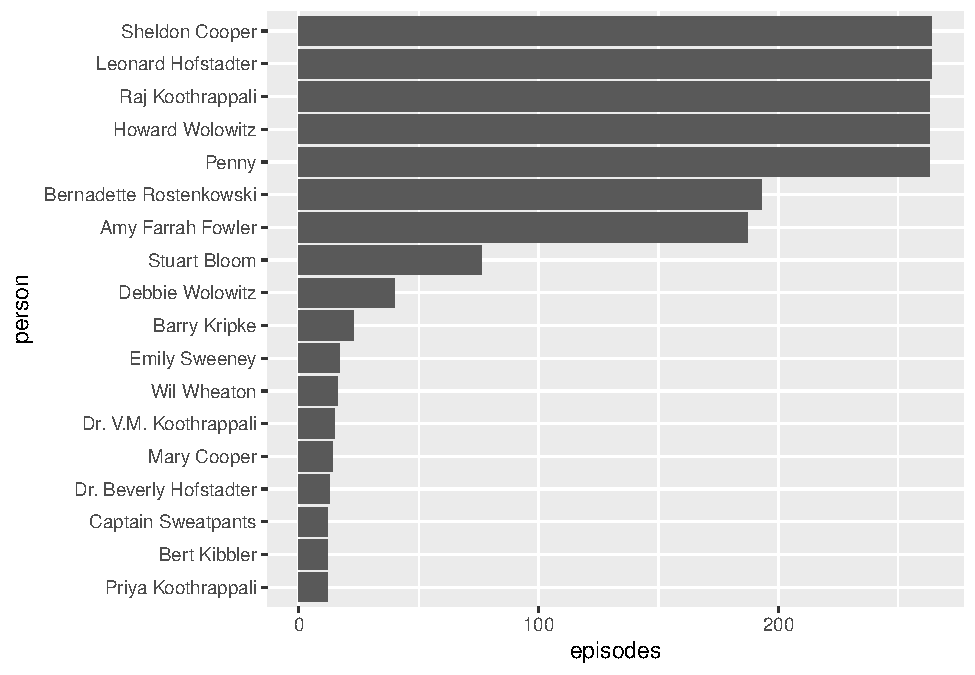
\includegraphics{getting-started_files/figure-latex/unnamed-chunk-23-1.pdf}

\chapter{Analyzing Data}\label{analyzing-data}

maybe we show a t-test here - bt no special packages

\chapter{Next Steps}\label{next-steps}

\section{How To Get Help}\label{how-to-get-help}

\begin{itemize}
\tightlist
\item
  Stack overflow
\end{itemize}

\section{More on packages}\label{more-on-packages}

\begin{itemize}
\tightlist
\item
  what goes here?
\end{itemize}

\section{Writting clean code}\label{writting-clean-code}

\begin{itemize}
\tightlist
\item
  We can reference some stuff here
\end{itemize}

\section{What else you can do with R}\label{what-else-you-can-do-with-r}

\begin{itemize}
\tightlist
\item
  dashboards
\item
  blogdown
\item
  deeplearning
\end{itemize}

\bibliography{book.bib,packages.bib}


\end{document}
